\documentclass{beamer}

\mode<presentation>
{

% The Beamer class comes with a number of default slide themes
% which change the colors and layouts of slides. Below this is a list
% of all the themes, uncomment each in turn to see what they look like.

%\usetheme{default}
%\usetheme{AnnArbor}
%\usetheme{Antibes}
%\usetheme{Bergen}
%\usetheme{Berkeley}
%\usetheme{Berlin}
%\usetheme{Boadilla}
%\usetheme{CambridgeUS}
%\usetheme{Copenhagen}
%\usetheme{Darmstadt}
%\usetheme{Dresden}
%\usetheme{Frankfurt}
%\usetheme{Goettingen}
%\usetheme{Hannover}
%\usetheme{Ilmenau}
%\usetheme{JuanLesPins}
%\usetheme{Luebeck}
\usetheme{Madrid}
%\usetheme{Malmoe}
%\usetheme{Marburg}
%\usetheme{Montpellier}
%\usetheme{PaloAlto}
%\usetheme{Pittsburgh}
%\usetheme{Rochester}
%\usetheme{Singapore}
%\usetheme{Szeged}
%\usetheme{Warsaw}

% As well as themes, the Beamer class has a number of color themes
% for any slide theme. Uncomment each of these in turn to see how it
% changes the colors of your current slide theme.

%\usecolortheme{albatross}
%\usecolortheme{beaver}
%\usecolortheme{beetle}
%\usecolortheme{crane}
%\usecolortheme{dolphin}
%\usecolortheme{dove}
%\usecolortheme{fly}
%\usecolortheme{lily}
%\usecolortheme{orchid}
%\usecolortheme{rose}
%\usecolortheme{seagull}
%\usecolortheme{seahorse}
%\usecolortheme{whale}
%\usecolortheme{wolverine}

%\setbeamertemplate{footline} % To remove the footer line in all slides uncomment this line
%\setbeamertemplate{footline}[page number] % To replace the footer line in all slides with a simple slide count uncomment this line

%\setbeamertemplate{navigation symbols}{} % To remove the navigation symbols from the bottom of all slides uncomment this line
}

\usepackage{graphicx} % Allows including images

\usepackage{booktabs} % Allows the use of \toprule, \midrule and \bottomrule in tables

\usepackage{mathtools}

\everymath{\displaystyle}

\usepackage{amssymb}

\usepackage{commath}

\usepackage{kantlipsum,graphicx}

\usepackage{amsmath}

\usepackage[utf8]{inputenc}

\usepackage{adjustbox}

\usepackage[customcolors,shadow,roundedcorners]{dynblocks}

\usepackage{tcolorbox}

\tcbuselibrary{theorems}

\tcbuselibrary{skins}

\usepackage{float}

%----------------------------------------------------------------------------------------
%	TITLE PAGE
%----------------------------------------------------------------------------------------

\title[Senior Thesis]{Singular Sturm-Liouville Eigenvalue Problems: \\Theory and Computation} % The short title appears at the bottom of every slide, the full title is only on the title page

\author{Brendan D. Busey and Stephen B. Robinson} % Your name

\institute[WFU] % Your institution as it will appear on the bottom of every slide, may be shorthand to save space
{

\includegraphics[scale=0.3]{WakeForestSeal1.png}

\vspace{3mm}

Wake Forest University \\ % Your institution for the title page
}

\date{\today} % Date, can be changed to a custom date

\begin{document}

\renewcommand\thesubsection{\thesection.\arabic{subsection}}

\renewcommand{\ttdefault}{cmtt}

\newtheorem{observation}{Observation}

\setbeamertemplate{theorems}[numbered]


%-------------------------------------------------------------------------------------------

%USED TO CREATE THE CUSTOM \begin{block} \end{block} lengths

%-------------------------------------------------------------------------------------------
\newenvironment<>{varblock}[2][.9\textwidth]{%
  \setlength{\textwidth}{#1}
  \begin{actionenv}#3%
    \def\insertblocktitle{#2}%
    \par%
    \usebeamertemplate{block begin}}
  {\par%
    \usebeamertemplate{block end}%
  \end{actionenv}}
  
%-----------------------------------------------------------------------------------------------

%USED TO MAKE ENUMERATED LISTS CONTINUE ACROSS SLIDES

%------------------------------------------------------------------------------------------------
\newcounter{sauvegardeenumi}

\newcommand{\asuivre}{\setcounter{sauvegardeenumi}{\theenumi}}

\newcommand{\suite}{\setcounter{enumi}{\thesauvegardeenumi}}

\begin{frame}

\titlepage

\end{frame}

\begin{frame}{Introduction}

\vspace*{-10mm}

\begin{itemize}

\item Throughout the research process, we studied the boundary value problem

\begin{center}

\begin{minipage}{6cm}

\begin{varblock}[6cm]

\begin{equation}
\begin{array}{l}
\displaystyle (-x^ny')'=\lambda x^my {~} in {~} (0,1)\\[2ex]
\displaystyle y(0)=0, y(1)=0 \\
\end{array} 
\label{eq:BVP}
\end{equation}

\end{varblock}

\end{minipage}

\end{center}

\end{itemize}

\begin{itemize}

\item Note: this boundary value problem is indeed an eigenvalue problem

\item With the following goals:

\begin{itemize}

\item determine the $\lambda$ values such that \eqref{eq:BVP} has a non-trivial solution

\item explore how the parameters $n$ and $m$ influence those eigenvalues

\end{itemize}

\end{itemize}

\end{frame}

\begin{frame}{Motivation}

\vspace*{-20mm}

\begin{itemize}

\item Our research is motivated by the work of Paul Binding and Hans Volkmer who, in $[1]$, discussed the following problem

\end{itemize}

\begin{block}

\begin{center}

$-(p(x)y')'+q(x)y=(\lambda r(x)+\mu)y,$ for $a \leq x \leq b$

\vspace{2mm}

with the separated boundary conditions

\vspace{2mm}

$\cos(\alpha)y(a)-\sin(\alpha)p(a)y'(a)=0$ and $\cos(\beta)y(b)-\sin(\beta)p(b)y'(b)=0$

\end{center}

\end{block}

\end{frame}

\begin{frame}{The Initial Value Problem}

\vspace*{-20mm}

\begin{itemize}

\item In order to gain a better understanding of $\eqref{eq:BVP}$, we investigated solutions to the following \textit{Initial Value Problem}

\begin{center}

\begin{minipage}{5cm}

\begin{varblock}[5cm]

\begin{equation}
\begin{array}{l}
\displaystyle (-x^ny')'=\lambda x^my\\[2ex]
\displaystyle y'(1)=-1, y(1)=0 \\
\end{array} 
\label{eq:IVP}
\end{equation}

\end{varblock}

\end{minipage}

\end{center}

\end{itemize}

\begin{itemize}

\item Defined on the interval $(0,1)$

\item Through experimentation, examined the affects of changing the value of $m$ and $n$ on the eigenvalues and eigenfunctions that were obtained

\end{itemize}

\end{frame}

\begin{frame}{Experimental research approach: The ``Shooting" Method}

\vspace*{-5mm}

Basic idea:

\vspace{2mm}

\begin{itemize}

\item Employed the mathematical software Maple in order to plot solutions of the Initial Value Problem \eqref{eq:IVP} for varying values of $m$, $n$, and $\lambda$ 

\end{itemize}

\begin{itemize}

\item Three situations

\end{itemize}

\begin{columns}

\column{0.2\textwidth}

``Overshoot"

\vspace{2mm}

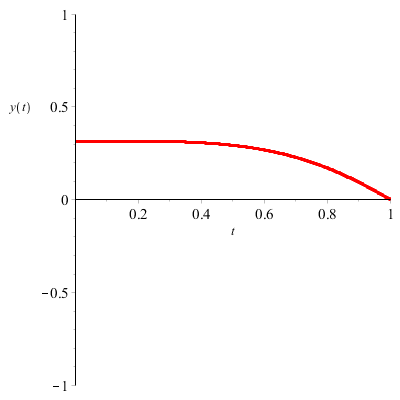
\includegraphics[scale=0.25]{Overshoot.png}

\column{0.2\textwidth}

``Undershoot"

\vspace{2mm}

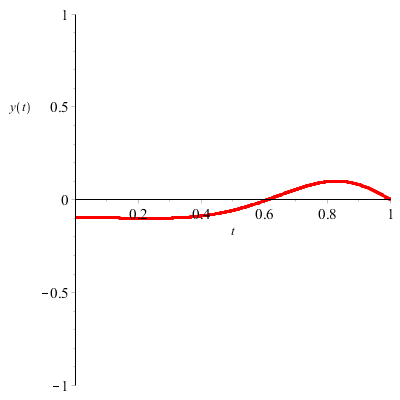
\includegraphics[scale=0.25]{Undershoot.png}

\column{0.2\textwidth}

``Just right"

\vspace{2mm}

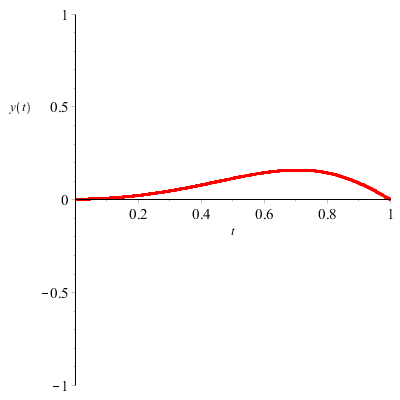
\includegraphics[scale=0.25]{JustRight.png}

\end{columns}

\end{frame}

\begin{frame}{First Experimental Result: No Eigenvalues}

\begin{columns}[T]

\hspace*{5mm}

\begin{column}{35mm}

\begin{itemize}

\item $n=2$, $m=0$, and $\lambda=4$

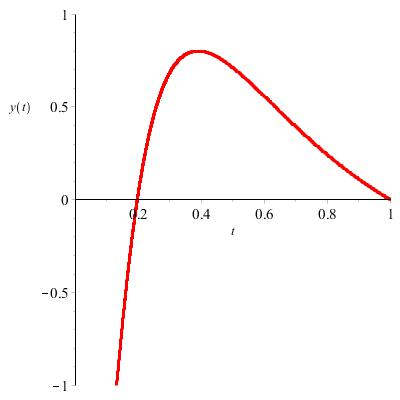
\includegraphics[scale=0.15]{NEquals2MEquals0LambdaEquals4}

\end{itemize}

\begin{itemize}

\item $n=2$, $m=0$, and $\lambda=7$

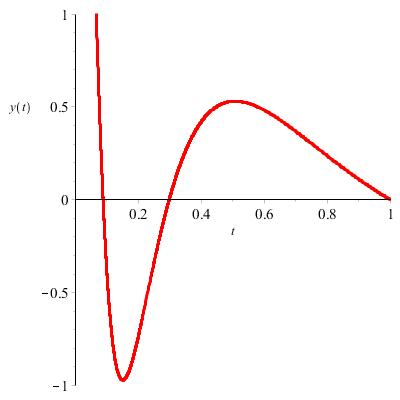
\includegraphics[scale=0.15]{NEquals2MEquals0LambdaEquals7}

\end{itemize}

\end{column}

\hspace*{5mm}

\begin{column}{35mm}

\begin{itemize}

\item $n=2$, $m=0$, and $\lambda=15$

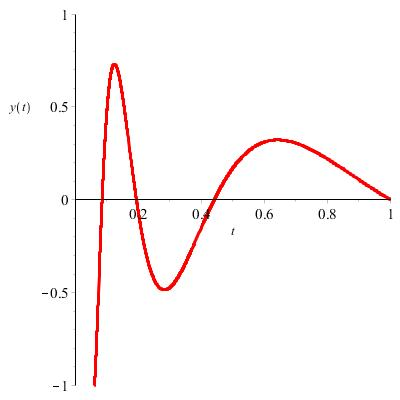
\includegraphics[scale=0.15]{NEquals2MEquals0LambdaEquals15}

\vspace{2.5mm}

\item $n=2$, $m=0$, and $\lambda=17$

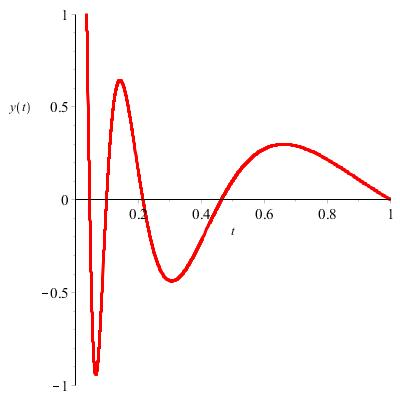
\includegraphics[scale=0.15]{NEquals2MEquals0LambdaEquals17}

\end{itemize}

\end{column}

\hspace*{-1mm}

\begin{column}{35mm}

\begin{itemize}

\item $n=2$, $m=0$, and $\lambda=22$

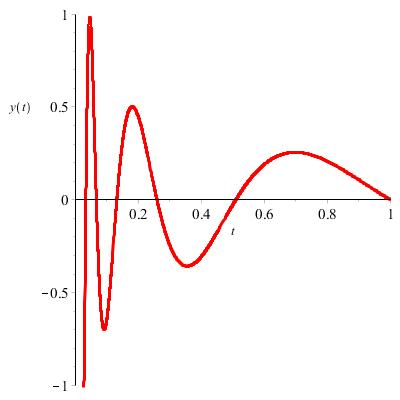
\includegraphics[scale=0.15]{NEquals2MEquals0LambdaEquals22}

\end{itemize}

\end{column}

\end{columns}

\end{frame}

\begin{frame}{First Theoretical Result: Euler Equations}

\vspace*{-10mm}

\begin{center}

\begin{observation}

For positive $m$ and $n$ values, asymptotic behaviour, specifically a vertical asymptote, occurs along the $x-axis$
 
\end{observation}

\end{center}

\vspace*{-5mm}

\begin{itemize}

\item We first considered solutions that were in the form of \textit{Euler equations}

\begin{itemize}

\item Are of the form $x^2y''+\alpha xy'+\beta y=0$, where $\alpha$ and $\beta$ are real constants

\item Have a point at which the Euler equation cannot be represented by a power series of the form $\sum_{n=0}^{\infty} a_{n} x^n$

\end{itemize}

\end{itemize}

\end{frame}

\begin{frame}{First Theoretical Result: Euler Equations (continued)}

Obtaining solutions:

\begin{enumerate}

\item We start with

\begin{center}

\begin{varblock}[12cm]

$(-x^ny')'=\lambda x^my$, subject to the boundary conditions $y(0)=0, y(1)=0$

\end{varblock}

\end{center}

\item Then, after computing derivatives and re-arranging we get

\begin{center}

\begin{minipage}{5cm}

\begin{varblock}[5cm]

$-x^ny''-nx^{n-1}y'-\lambda x^my=0$

\end{varblock}

\end{minipage}

\end{center}

\item We next suppose that solutions are of the form $y=x^r$, calculate more derivatives, plug-in our derivatives appropriately, and after some algebra, we have

\begin{center}

\begin{minipage}{10cm}

\begin{varblock}[10cm]

$r(r-1)+nr+\lambda=0$, which is our \textit{characteristic} equation

\end{varblock}

\end{minipage}

\end{center}

\asuivre

\end{enumerate}

\end{frame}

\begin{frame}{First Theoretical Result: Euler Equations (continued)}

\begin{enumerate}

\suite

\item We use the quadratic formula after plugging in our well-chosen value of $n=-1$ to find the roots of our characteristic equation

\begin{center}

\begin{minipage}{3cm}

\begin{varblock}[3cm]

$\frac{-1}{2} \pm \sqrt{\frac{1}{4}-\lambda}$

\end{varblock}

\end{minipage}

\end{center}

\item Finally, after some substitution, using our initial conditions, and using \textit{Euler's formula} to extract the real (non-complex) roots, we have our final solutions

\begin{center}

\begin{minipage}{6cm}

\begin{varblock}[6cm]

$y_{1}(x)=x^{-\frac{1}{2}}\cos\bigg(\sqrt{\lambda-\frac{1}{4}} \ln(x)\bigg)$

\end{varblock}

\end{minipage}

\end{center}

\begin{center}

\begin{minipage}{6cm}

\begin{varblock}[6cm]

$y_{2}(x)=x^{-\frac{1}{2}}sin\bigg(\sqrt{\lambda-\frac{1}{4}} \ln(x)\bigg)$

\end{varblock}

\end{minipage}

\end{center}

\end{enumerate}

\end{frame}

\begin{frame}{Second Experimental Result: Existence of Eigenvalues}

\begin{columns}[T]

\hspace*{-3mm}

\begin{column}{35mm}

\begin{itemize}

\item $n=-1$, $m=1$, and $\lambda=39$

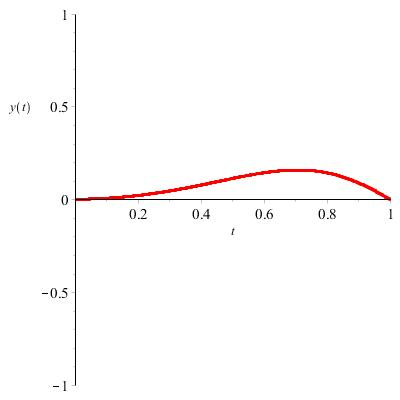
\includegraphics[scale=0.2]{NEqualsNegative1MEquals1LambdaEquals39}

\end{itemize}

\begin{itemize}

\vspace*{-3mm}

\item $n=-1$, $m=1$, and $\lambda=160$

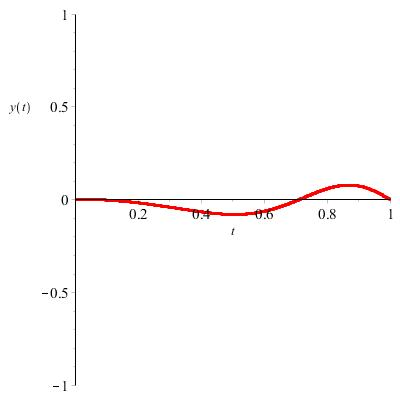
\includegraphics[scale=0.2]{NEqualsNegative1MEquals1LambdaEquals160}

\end{itemize}

\end{column}

\hspace*{-3mm}

\begin{column}{35mm}

\begin{itemize}

\item $n=-1$, $m=1$, and $\lambda=355$

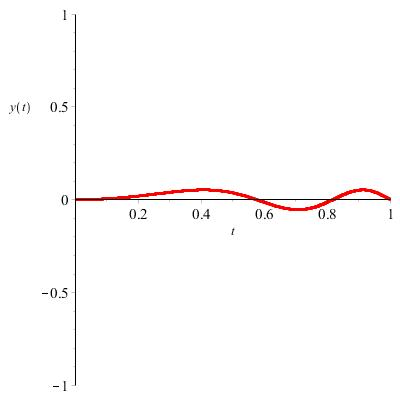
\includegraphics[scale=0.2]{NEqualsNegative1MEquals1LambdaEquals355}

\item $n=-1$, $m=1$, and $\lambda=640$

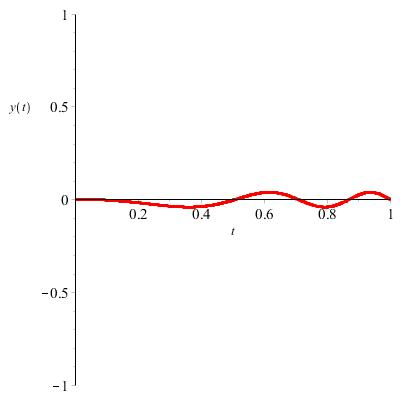
\includegraphics[scale=0.2]{NEqualsNegative1MEquals1LambdaEquals640}

\end{itemize}

\end{column}

\hspace*{-7mm}

\begin{column}{35mm}

\begin{itemize}

\item $n=-1$, $m=1$, and $\lambda=990$

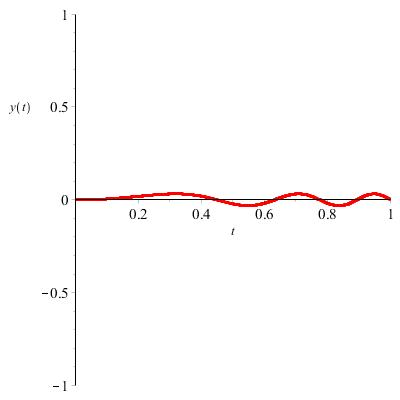
\includegraphics[scale=0.2]{NEqualsNegative1MEquals1LambdaEquals990}

\end{itemize}

\end{column}

\end{columns}

\end{frame}

\begin{frame}{Second Theoretical Result: Power Series Solutions and the Method of Frobenius}

\begin{observation}

When $m$ is greater than $n$, $n$ is negative or zero, and as lambda values increase, the roots become clustered closer together.
 
\end{observation}

\begin{itemize}

\item Previously, we had considered finding solutions using \textit{Euler equations}

\begin{center}

\begin{minipage}{9cm}

\begin{varblock}[9cm]

$x^2y''+\alpha xy'+\beta y=0$, where $\alpha$ and $\beta$ are real constants

\end{varblock}

\end{minipage}

\end{center}

\item With the method of Frobenius, however, we replace $\alpha$ and $\beta$ in the above equation with coefficients that have ``nice" series representations

\begin{center}

\begin{minipage}{6cm}

\begin{varblock}[6cm]

$x^2y'' + x[\alpha(x)]y' + [\beta(x)]y=0$

\end{varblock}

\end{minipage}

\end{center} 

\end{itemize}

\end{frame}

\begin{frame}{Second Theoretical Result: Power Series Solutions and the Method of Frobenius (continued)}

Deriving solutions:

\begin{enumerate}

\item As before, we begin with

\begin{center}

\begin{varblock}[12cm]

$(-x^ny')'=\lambda x^my$, subject to the boundary conditions $y(0)=0, y(1)=0$

\end{varblock}

\end{center}

\item Then, after computing derivatives and re-arranging we get

\begin{center}

\begin{minipage}{5cm}

\begin{varblock}[5cm]

$-x^ny''-nx^{n-1}y'-\lambda x^my=0$

\end{varblock}

\end{minipage}

\end{center}

\item If we make the substitution for our well-chosen values of $n=-1$ and $m=1$, multiply through by $x^3$, and simplify, we have

\begin{center}

\begin{minipage}{4cm}

\begin{varblock}[4cm]

$x^2y''-xy'+\lambda x^4y=0$

\end{varblock}

\end{minipage}

\end{center}

\asuivre

\end{enumerate}

\end{frame}

\begin{frame}{Second Theoretical Result: Power Series Solutions and the Method of Froenius (continued)}

\begin{enumerate}

\suite

\item Then, if we compare the general equation

\begin{center}

\begin{minipage}{6cm}

\begin{varblock}[6cm]

$x^2y'' + x[\alpha(x)]y' + [\beta(x)]y=0$

\end{varblock}

\end{minipage}

\end{center}

With our equation

\begin{center}

\begin{minipage}{4cm}

\begin{varblock}[4cm]

$x^2y''-xy'+\lambda x^4y=0$

\end{varblock}

\end{minipage}

\end{center}

It is clear that

\begin{center}

\begin{minipage}{6cm}

\begin{varblock}[6cm]

$\alpha(x)=-1$ $\quad$ and $\quad$ $\beta(x)=\lambda x^4$

\end{varblock}

\end{minipage}

\end{center}

\item Then, we confirm that the point $x=0$ is indeed a regular singular point by computing the following limits and showing that they exist

\begin{center}

\begin{minipage}{7cm}

\begin{varblock}[7cm]

$\lim_{x \to 0} \alpha(x)=-1$ $\quad$ and $\quad$ $\lim_{x \to 0} \beta(x)=0$

\end{varblock}

\end{minipage}

\end{center}

\asuivre

\end{enumerate}

\end{frame}

\begin{frame}{Second Theoretical Result: Power Series Solutions and the Method of Frobenius (continued)}

\begin{enumerate}

\suite

\item Now that we have shown that $x=0$ is a regular singular point, we know that our solutions will be of the form

\begin{center}

\begin{minipage}{4cm}

\begin{varblock}[4cm]

$y(x)=x^r \sum_{n=0}^{\infty} a_{n} x^n$

%$\alpha(x)=\sum_{n=0}^{\infty} p_{n} x^{n}$ $\quad$ and $\quad$ $\beta(x)=\sum_{n=0}^{\infty} q_{n} x^{n}$

\end{varblock}

\end{minipage}

\end{center}

\item We also know that $\alpha(x)$ and $\beta(x)$ can be defined as follows

 \begin{center}

\begin{minipage}{8cm}

\begin{varblock}[8cm]

$\alpha(x)=\sum_{n=0}^{\infty} p_{n} x^{n}$ $\quad$ and $\quad$ $\beta(x)=\sum_{n=0}^{\infty} q_{n} x^{n}$

\end{varblock}

\end{minipage}

\end{center}

\item Similar to the \textit{characteristic equation} we had with Euler equations, here, we have our \textit{indicial equation}

\begin{center}

\begin{minipage}{5cm}

\begin{varblock}[5cm]

$F(r)=r(r-1)+p_{0}r+q_{0}=0$

\end{varblock}

\end{minipage}

\end{center}

\asuivre

\end{enumerate}

\end{frame}

\begin{frame}{Second Theoretical Result: Power Series Solutions and the Method of Frobenius (continued)}

\begin{enumerate}

\suite

\item If we then evaluate $\alpha(x)=\sum_{n=0}^{\infty} p_{n} x^{n}$ and $\beta(x)=\sum_{n=0}^{\infty} q_{n} x^{n}$ at $n=0$, plug this into our \textit{indicial equation}, and solve for $r$, we find

\begin{center}

\begin{minipage}{4cm}

\begin{varblock}[4cm]

$r_{1}=2$ $\quad$ and $\quad$ $r_{2}=0$

\end{varblock}

\end{minipage}

\end{center}

\item At this point, we know that our solutions will be of the form

\begin{center}

\begin{minipage}{6cm}

\begin{varblock}[6cm]

$y_{1}(x)=\abs{x}^{r_{1}} \bigg[1 + \sum_{n=1}^{\infty} a_{n}(r_{1})x^n\bigg]$

\end{varblock}

\end{minipage}

\end{center}

and

\begin{center}

\begin{minipage}{8cm}

\begin{varblock}[8cm]

$y_{2}(x)=ay_{1}(x) \ln{\abs{x}} + \abs{x}^{r_{2}} \bigg[1 + \sum_{n=1}^{\infty} c_{n}(r_{2})x^n\bigg]$

\end{varblock}

\end{minipage}

\end{center}

\asuivre

\end{enumerate}

\end{frame}

\begin{frame}{Second Theoretical Result: Power Series Solutions and the Method of Frobenius (continued)}

\vspace*{-15mm}

\begin{enumerate}

\suite

\item Finally, after substituting in for $r_{1}$, $r_{2}$, and $y_{1}(x)$ and simplifying

\begin{center}

\begin{minipage}{5cm}

\begin{varblock}[5cm]

$y_{1}(x)=\abs{x}^{2} \bigg[1 + \sum_{n=1}^{\infty} 2a_{n}x^n\bigg]$

\end{varblock}

\end{minipage}

\end{center}

and

\begin{center}

\begin{minipage}{7cm}

\begin{varblock}[7cm]

$y_{2}(x)=a \abs{x}^{2} \bigg[1 + \sum_{n=1}^{\infty} 2a_{n}x^n\bigg] \ln{\abs{x}} + 1$

\end{varblock}

\end{minipage}

\end{center}

\end{enumerate}

\end{frame}

\begin{frame}{Future ideas}

\begin{enumerate}

\vspace*{-40mm}

\item Explore a greater variety of values for $m$ and $n$

\item Investigate fractional differences between $m$ and $n$

\end{enumerate}

\end{frame}

\begin{frame}{Acknowledgements}

\vspace*{-40mm}

I would like to thank Dr. Robinson as well as the entire Mathematics department for all their help and support.

\end{frame}

\begin{frame}{References}

\vspace*{-20mm}

\begin{center}

\begin{thebibliography}{9}

\bibitem{EigencurvesForTwoParameter} 
Binding, Paul; Volkmer, Hans
\textit{Eigencurves for two-parameter Sturm-Liouville equations. SIAM Rev. 38 (1996), no. 1, 27---48}.

\vspace{1mm}

\bibitem{ElementaryDifferentialEquationsAndBoundaryValueProblems}
Boyce, William E.; DiPrima, Richard C.
\textit{Elementary differential equations and boundary value problems. John Wiley \& Sons, Inc., New York-London-Sydney 1965 xi+485 pp. 34.00}. 

\end{thebibliography}

\end{center}

\end{frame}

\end{document}